\section{Evaluation}
\label{sec:evaluation}

\subsection{Qualitative scenarios}
\label{subsec:scenarios}

Five scenarios exercise distinct failure modes, run on
GPT-4o-2024-08-06 with \texttt{logprobs=True, top\_logprobs=5} and a
system prompt specifying concise naming conventions.

\paragraph{A --- Deprecated API (Stripe).}
\textit{``Charge a customer's card for \$50.''} $\eps = 0.914$,
\textsc{paused}. The peak token is the method selector after
\texttt{stripe}: \texttt{.Ch} (\texttt{Charge}, prob.\ $0.52$) vs.\
\texttt{.Payment} (\texttt{PaymentIntent}, prob.\ $0.47$). Both paths
are in the training data; neither is definitively preferred.

\paragraph{B --- Confident wrongness (OpenAI SDK).}
\textit{``Call GPT-4 and return the response text.''} $\eps = 0.551$,
\textsc{flagged}. The model generated v0
(\texttt{openai.ChatCompletion.create(\ldots)}) confidently; v0 raises
\texttt{AttributeError} on SDK $\ge 1.0$. \eps fired not on the API
call --- the model was certain --- but on surrounding parameter
design. \textsc{flagged} routes the function to the review loop; the reviewer,
examining the full function, surfaces the deprecated call. This is
indirect detection: \eps flagged adjacent uncertainty, not the failing
token itself.

\paragraph{C --- Syntax split (SQLAlchemy).}
\textit{``Query all active users.''} $\eps = 0.435$, \textsc{flagged}.
The model chose 1.x (\texttt{db.query(User).filter(\ldots)}); primary
flag was the import path. \textsc{flagged} (not \textsc{paused})
reflects preference without certainty.

\paragraph{D --- Compatibility mismatch (FastAPI async/sync).}
\textit{``FastAPI endpoint that fetches weather from an external
API.''} $\eps = 0.812$, \textsc{paused}. The model generated
\texttt{async def} with \texttt{requests.get()} inside --- two
individually defensible decisions (\texttt{async} $\eps = 0.26$,
\texttt{requests} $\eps = 0.31$) that combine into a silent bug
(blocks the event loop). \eps did not fire on the async/sync
combination directly; the \textsc{paused} flag came from URL/key
handling elsewhere in the file. A mismatch post-processor, run on
already-flagged functions, surfaced the combination explicitly ---
arguing for cross-decision consistency checks as a complement to \eps.

\paragraph{E --- Multi-function module.}
Six auth functions with four interdependent decisions (password hash,
JWT, SQLAlchemy, datetime). \textsc{paused} on all 16 runs,
$\eps \in [0.69, 0.92]$. Library choices varied across runs (passlib,
bcrypt, PyJWT, python-jose, mixed), but each run looked internally
confident. Early functions $\eps = 0.40$--$0.58$; later functions
frequently $\eps = 0.000$ --- an \emph{uncertainty collapse} after
initial commitment. The first function is the high-risk window.

\begin{figure}[H]
\centering
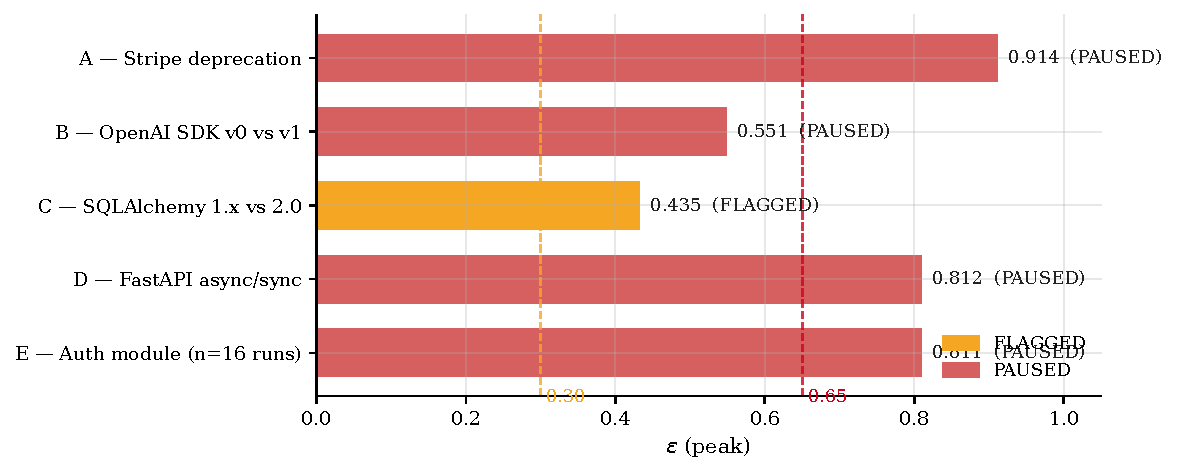
\includegraphics[width=0.85\textwidth]{figures/fig3_scenarios.pdf}
\caption{Scenarios A--E summarised by failure class and peak $\eps$.
All five clear the \textsc{flagged} threshold; four cross \textsc{%
paused}, giving the developer a single scalar urgency signal per
failure mode.}
\label{fig:scenarios}
\end{figure}

\subsection{Scenario E limitation: joint-prompt uncertainty collapse}
\label{subsec:scenarioE}

Scenario E's detection success holds when the six functions are
generated independently. When generated in a \emph{single} prompt with
``use a consistent library,'' \eps collapses across all six functions
--- not just the later ones. The joint signature list plus the
consistency instruction resolves the library choice before decoding
starts, leaving nothing for \eps to observe
(Table~\ref{tab:scenarioE}, GPT-4o-mini).

\begin{table}[h]
\centering
\small
\begin{tabular}{lrr}
\toprule
Function & Combined peak \eps & Per-function peak \eps \\
\midrule
\texttt{register\_user}          & $0.579$ & $0.627$ \\
\texttt{login}                   & $0.820$ & $0.872$ \\
\texttt{verify\_token}           & $0.606$ & $0.911$ \\
\texttt{refresh\_token}          & $0.414$ & $0.711$ \\
\texttt{request\_password\_reset}& $0.295$ & $0.788$ \\
\texttt{reset\_password}         & $0.394$ & $0.728$ \\
\bottomrule
\end{tabular}
\caption{Combined generation collapses \eps for every function.
DeepSeek V3 shows the same pattern. When context resolves uncertainty
before decoding, there is nothing for \eps to observe.}
\label{tab:scenarioE}
\end{table}

\begin{figure}[H]
\centering
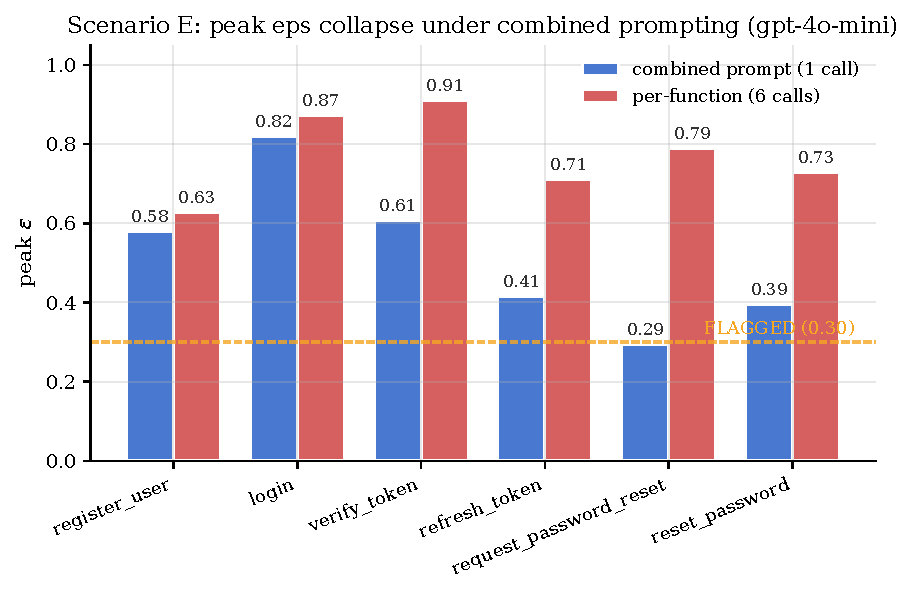
\includegraphics[width=0.85\textwidth]{figures/fig8_scenario_e.pdf}
\caption{Per-function generation keeps three of six functions above
\textsc{flagged}; combined generation pushes four below it. The
detector is honest about what is resolved prior to decoding.}
\label{fig:scenarioE}
\end{figure}

\subsection{Multi-model calibration}
\label{subsec:calibration}

A 30-prompt calibration set: 10 LOW prompts (sort, palindrome,
fibonacci, two-sum --- pure logic) and 20 HIGH prompts
(API/version-split tasks across Stripe, OpenAI, SQLAlchemy, FastAPI,
Pydantic), run on three models. GPT-4o achieves $85\%$ HIGH detection
at $50\%$ LOW FP; GPT-4o-mini and GPT-4-turbo both achieve $70\%$ at
$60\%$ LOW FP.

\begin{table}[h]
\centering
\small
\begin{tabular}{lrr}
\toprule
Model & HIGH detection & LOW FP \\
\midrule
GPT-4o      & $85\%$ (17/20) & $50\%$ (5/10) \\
GPT-4o-mini & $70\%$ (14/20) & $60\%$ (6/10) \\
GPT-4-turbo & $70\%$ (14/20) & $60\%$ (6/10) \\
\bottomrule
\end{tabular}
\caption{Calibration at the \textsc{flagged} threshold ($\eps \ge
0.30$). $95\%$ Wilson CIs: $\pm 17$pp HIGH, $\pm 30$pp LOW. GPT-4o's
lead correlates with better logprob calibration. Three prompts produce
$\eps = 0.000$ across all models --- \emph{confidently-resolved
domains} where training priors have converged.}
\label{tab:calibration}
\end{table}

\subsection{LOW ground truth}
\label{subsec:low-gt}

All 30 LOW functions passed \texttt{exec()} assertions. Tier
breakdown: \textsc{complete} $5$, \textsc{flagged} $11$,
\textsc{paused} $9$, \textsc{aborted} $5$. Non-\textsc{complete} tiers
are dominated by Type 3 (brute vs.\ hash two-sum; recursive vs.\
iterative fibonacci).

\subsection{Precision/recall at tier boundaries}
\label{subsec:pr}

On a 200-entry combined set (30 LOW exec-verified plus 170 HIGH
LLM-judged; see~\S\ref{subsec:gt-disclosure}), 53 true failures and
147 correct:

\begin{table}[h]
\centering
\small
\begin{tabular}{lrrr}
\toprule
Threshold & Precision & Recall & F1 \\
\midrule
$\eps \ge 0.30$ (\textsc{flagged+}) & $0.272$ & $\mathbf{1.000}$ & $0.428$ \\
$\eps \ge 0.65$ (\textsc{paused+})  & $0.293$ & $0.868$ & $\mathbf{0.438}$ \\
$\eps \ge 0.95$ (\textsc{aborted})  & $0.309$ & $0.547$ & $0.394$ \\
\bottomrule
\end{tabular}
\caption{$n=200$, $53$ positives; $95\%$ Wilson CI on
\textsc{flagged+} precision $[0.22, 0.33]$. Base failure rate $26.5\%
\approx$ \textsc{flagged+} precision: the gate's value is recall, not
precision. HIGH ground truth for $170/200$ entries is LLM-judged by
GPT-4o (\S\ref{subsec:gt-disclosure}); LOW ground truth ($30/200$)
is \texttt{exec()}-verified.}
\label{tab:pr}
\end{table}

\begin{figure}[H]
\centering
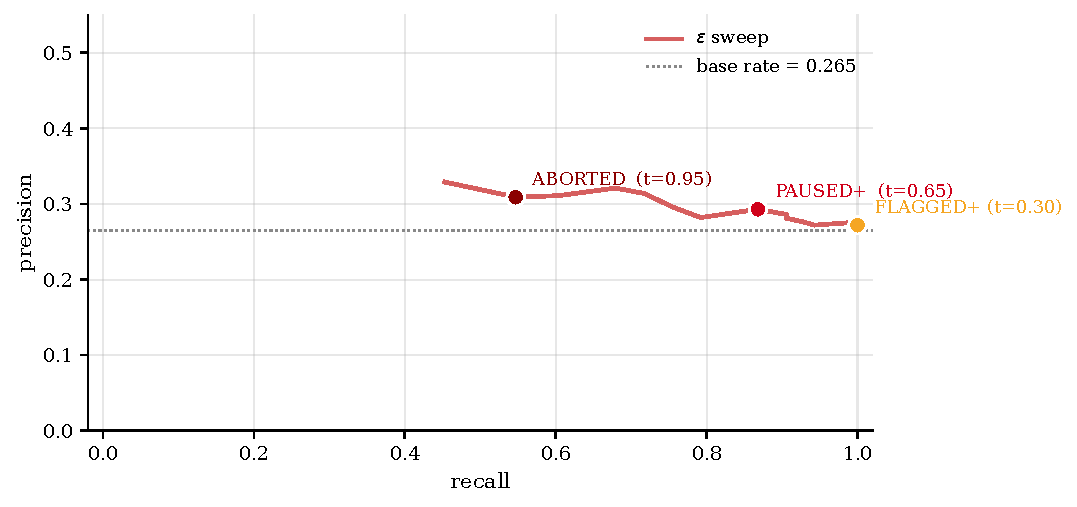
\includegraphics[width=0.85\textwidth]{figures/fig6_pr_curve.pdf}
\caption{Precision stays near the base rate across the threshold
range; recall falls monotonically. At \textsc{flagged+}, recall is
$1.00$ at precision barely above base rate --- the gate's value is
recall, not precision.}
\label{fig:pr-curve}
\end{figure}

Tier monotonicity is modest ($27\%/29\%/31\%$); tiers are urgency
signals, not calibrated probabilities. The useful binary boundary is
\textsc{complete} vs.\ \textsc{flagged+}.

\subsection{Review loop: context-free vs.\ context-primed reviewer}
\label{subsec:review-loop}

Evaluated on 201 entries (production FastAPI codebase plus scenarios
A--E, three models). Every \textsc{flagged+} entry is sent in
parallel to a GPT-4o reviewer returning \textsc{cleared}/\textsc{%
confirmed}; a consolidation pass processes remaining suspects.
The \textbf{context-free} variant uses no reviewer context; the \textbf{context-primed} variant injects model-%
specific learned false-positive patterns from a prior clean run (injecting suspect
patterns caused over-flagging in pilots).

\begin{table}[h]
\centering
\small
\begin{tabular}{lrr}
\toprule
Metric & Context-free & Context-primed \\
\midrule
Cleared by reviewer        & $107/201$ ($53.2\%$) & $138/201$ ($68.7\%$) \\
Forwarded to consolidation & $89$                 & $57$ \\
Confirmed true failures    & $85$ ($42.3\%$)      & $57$ ($28.4\%$) \\
Late false positives       & $4$                  & $0$ \\
\bottomrule
\end{tabular}
\caption{``Late false positive'' = an entry marked \textsc{confirmed}
that was in fact correct on manual inspection. The context-primed variant is the preferred
production configuration.}
\label{tab:review}
\end{table}

\begin{figure}[H]
\centering
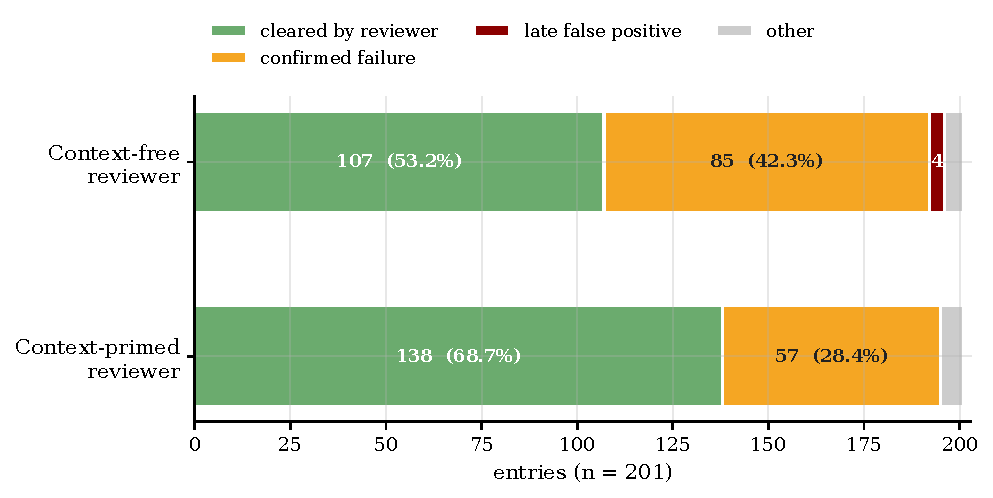
\includegraphics[width=0.85\textwidth]{figures/fig7_review_loop.pdf}
\caption{Injecting learned FP patterns into the reviewer (context-primed
vs.\ context-free) shifts $31$ additional entries from consolidation to
cleared and eliminates late false positives, at the cost of suppressing
some true failures the context-free reviewer forwarded.}
\label{fig:review-loop}
\end{figure}

End-to-end failure rates: GPT-4o-mini $40\%$, GPT-4o $29\%$, DeepSeek
V3 $26\%$. Because stage-1 recall is $100\%$, end-to-end precision is
determined entirely by the reviewer's precision on the \textsc{flagged+}
set. The context-primed variant's zero late-FP result rests on $n=57$ confirmed entries and
needs a larger validation study. The stage-1 recall guarantee applies
to entries that reach the reviewer; entries the reviewer clears were
not independently verified.

